\documentclass[conference]{IEEEtran}
\usepackage{amsmath}
\usepackage{graphicx}
\usepackage{hyperref}
\usepackage{array}

\title{Advanced Network Scanner}
\author{
    Dipesh Kumar Kushwaha\\
    \texttt{221FA19067@vignan.ac.in}
    \and
    Saugat Chaudhary\\
    \texttt{221FA19066@vignan.ac.in}
    \and
    G. Vineela\\
    \texttt{221FA19022@vignan.ac.in}
    \and
    B. Suchentha\\
    \texttt{221FA19004@vignan.ac.in} 
    \and
    \\
    \\
    We would like to express our heartfelt gratitude to our guide, Dr.\\ Radha Rani, for her invaluable guidance, encouragement, and support\\ throughout the development of this project. Her expertise and\\ insights greatly contributed to the successful completion of this\\ work.\\
}

\date{\today}



\begin{document}



\maketitle

\begin{abstract}
\textbf{It finds weaknesses in network devices, which helps reinforce organizational security policies. Regular scanning helps identify and reveal security gaps, thus protecting networks and systems from exploitation that might result in data loss or compromise of devices.
This dissertation will talk about two open-source scanners, namely NMAP, Bettercap, and OpenVAS. Their individual features will be analyzed. Both were then integrated in a user-friendly GUI. Comprehensive information in the paper is reliable, since there are crucial points in examining the network being studied by these tools, though their heterogeneity as well as the complexity in data analyzing are some limitations of those tools. Therefore, in this paper, a new network scanner has been created to combine all the facilities of NMAP and to overcome some limitations of this tool. This scanner identifies active hosts, determines their operating systems and installed programs, and detects open ports and running services.}

\textbf{It goes beyond mere scanning because it is meant to make vulnerability assessment against a given vulnerability signature database by comparison of collected network data, listing possible threats. The feature also has auto-scanning of compromised devices so that ongoing monitoring and testing can occur, providing features such as network mapping, categorizing the types of vulnerabilities identified, and detecting configuration faults. It offers a far more streamlined assessment of vulnerability and significantly cuts down scan time.}

\end{abstract}

\section{Introduction}
With the world becoming more and more connected through the internet and networking technologies, network security has become very important. Organizations are moving business functions to public networks, putting huge amounts of personal, commercial, and organizational data at risk. This openness exposes systems to threats from external hackers or malicious insiders who can compromise sensitive information, affecting an organization's competitiveness and security.

Network security is used in the protection of intellectual property and in maintaining data integrity. Techniques involved in network security include network scanning and vulnerability assessment. Network scanning identifies active hosts in a network, which provide foundational data on the state of computer systems for security assessments. Vulnerability assessment systematically evaluates the security status of information systems, indicating weaknesses that could be exploited.

Network scanning and vulnerability assessment are a comprehensive approach to auditing, penetration testing, reporting, and patching that enable organizations to better protect their networks against potential threats.

\section{Related Work}
There are many tools in the market today. These tools are widely used because they are open source and give best results.
\\• Network mapping with NMAP
\\• Vulnerability assessment with OpenVAS
\\• Network mapping with bettercap, ethercap, wireshark, etc.


\subsection{Network mapping with NMAP}
NMAP ("Network Mapper") is one of the free, open-source utilities for network and security auditing. A lot of system and network administrators also consider network inventory, managing service update schedules, and uptime hosting to be important tasks as well. NMAP makes use of raw IP packets as part of innovative techniques to discover what hosts are reachable on the network, what services (application name and version) those hosts were providing, what operating systems (and OS versions) they were running, what type of packet filters/firewalls were in place, and much more. It was designed to quickly scan large networks, but performs well against single hosts. NMAP natively runs on all major computer operating systems. In addition to the great charge line NMAP executable, the NMAP suite also includes a developed GUI and results viewer (Zenmap), a flexible data transfer, redirection, and debugging tool (Ncat), a utility for scanning results comparison (Ndiff), and a packet generating and response analysis tool (Nping).

\textbf{Advantages of NMAP:}
\\• Unlimited IP scanning.
\\• Easy to setup and use.
\\• Fast Scans
\\•  Customizable Scans

\begin{figure}[h]
    \centering
    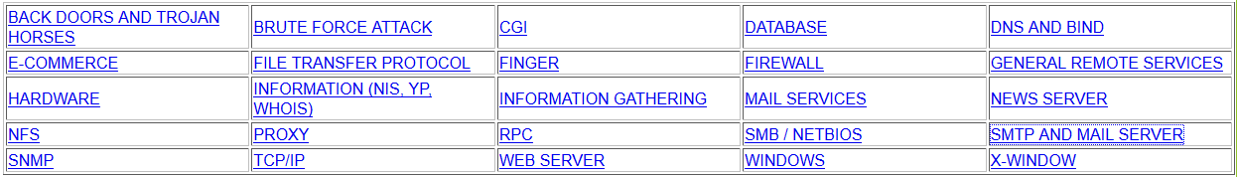
\includegraphics[width=1\linewidth]{image.png}
    \caption{Overview of NMAP}
    \label{1}
\end{figure}

\textbf{Disadvantage of NMAP:}

In the already crowded market of vulnerability scanners, NMAP may not receive the development focus it needs to stay current.

\subsection{OpenVAS}
Open Vulnerability Assessment System or OpenVAS is a skeleton of several tools as well as services offering a far-reaching and influential vulnerability scanning and vulnerability management solution. The security scanner comes along with the day-to-day updated feed of Network Vulnerability Tests, more than 30,000 in total as of April 2013. OpenVAS is a "remote scanner" because of the fact that it does not have to be introduced on a target for it to test; instead, it could be installed and configured on one and only device and test many hosts. OpenVAS has a client-server architecture over SSL.

\textbf{The architecture in figure 2 is explained below:}

\textit{
• The core of the architecture is the OpenVAS scanner, which executes the NVTs. The NVT feeds are regularly updated for the tests.
\\• OpenVAS manager: It offers the integration of vulnerability scanning and vulnerability management. The administrator makes it feasible to implement several customers for consistent behavior. It also controls a SQL database for central storage.
\\• Greenbone security desktop: GSD provides a desktop client.
\\• OpenVAS CLI: This is a command-line based utility.
}
\begin{figure}[h]
    \centering
    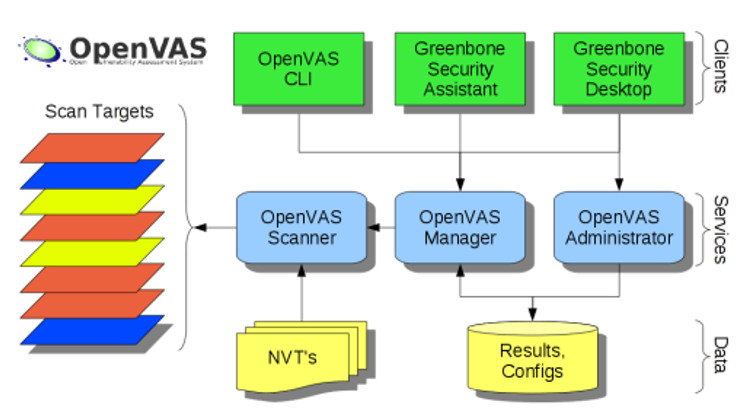
\includegraphics[width=1\linewidth]{openvas.png}
    \caption{Architecture of OpenVAS}
    \label{fig:enter-label}
\end{figure}

\begin{figure}[h]
    \centering
    \includegraphics[width=1\linewidth]{working of openvas.png}
    \caption{Working of OpenVas}
\end{figure}

\subsubsection{Working of OpenVAS:}
Most high-level network traffic-for example, websites, email, and so forth-arrives at a server via a high-level protocol carried in a TCP stream. To prevent a multiplicity of streams from interfering with each other, a computer divides its physical connection to the network into thousands of logical paths, known as ports. Each computer or device has various ports, and each could have a service running against it (i.e., a server for a specific protocol listening on it). OpenVAS works by checking one port on a computer, trying to determine which service that is running on, then proceeds to test that service and check if any vulnerabilities within this service are exploitable by the attacker against the computer.



\textbf{Advantages of OpenVAS:}
\\• Free, limitless IPs.
\\• Community support
\\• It can present an audit report.
\\• Demonstrates history of scanning.
\\• Experienced and endorsed by consultants directly working for the US Government. Used by the Government of Germany.

\textbf{Disadvantage of OpenVAS:}
\\• It is very complex to install and configure.

\subsection{betterCAP:}
BetterCAP is a powerful modular, extensible tool made specifically for network security and penetration testing, especially for man-in-the-middle attacks. It was initially developed to be an alternative solution when tools such as Ettercap are not available since it assists users in the monitoring, injection, as well as modification of traffics in a network, with other areas being ethical hacking and other network security-related areas.

\subsubsection{Working of betterCAP: }

BetterCAP works by intercepting traffic between a user and the destination server, positioning it in the middle. How it works in simple words is as follows:


\\• Packet Sniffing: Listens to and captures network packets to gather information on devices and traffic.
\\• ARP Spoofing: Sends fake ARP messages to act as the network gateway, intercepting traffic from all devices.
\\• DNS Spoofing: Redirects a user's DNS query to an attacker-controlled IP, leading users to malicious sites.
\begin{figure}[h]
    \centering
    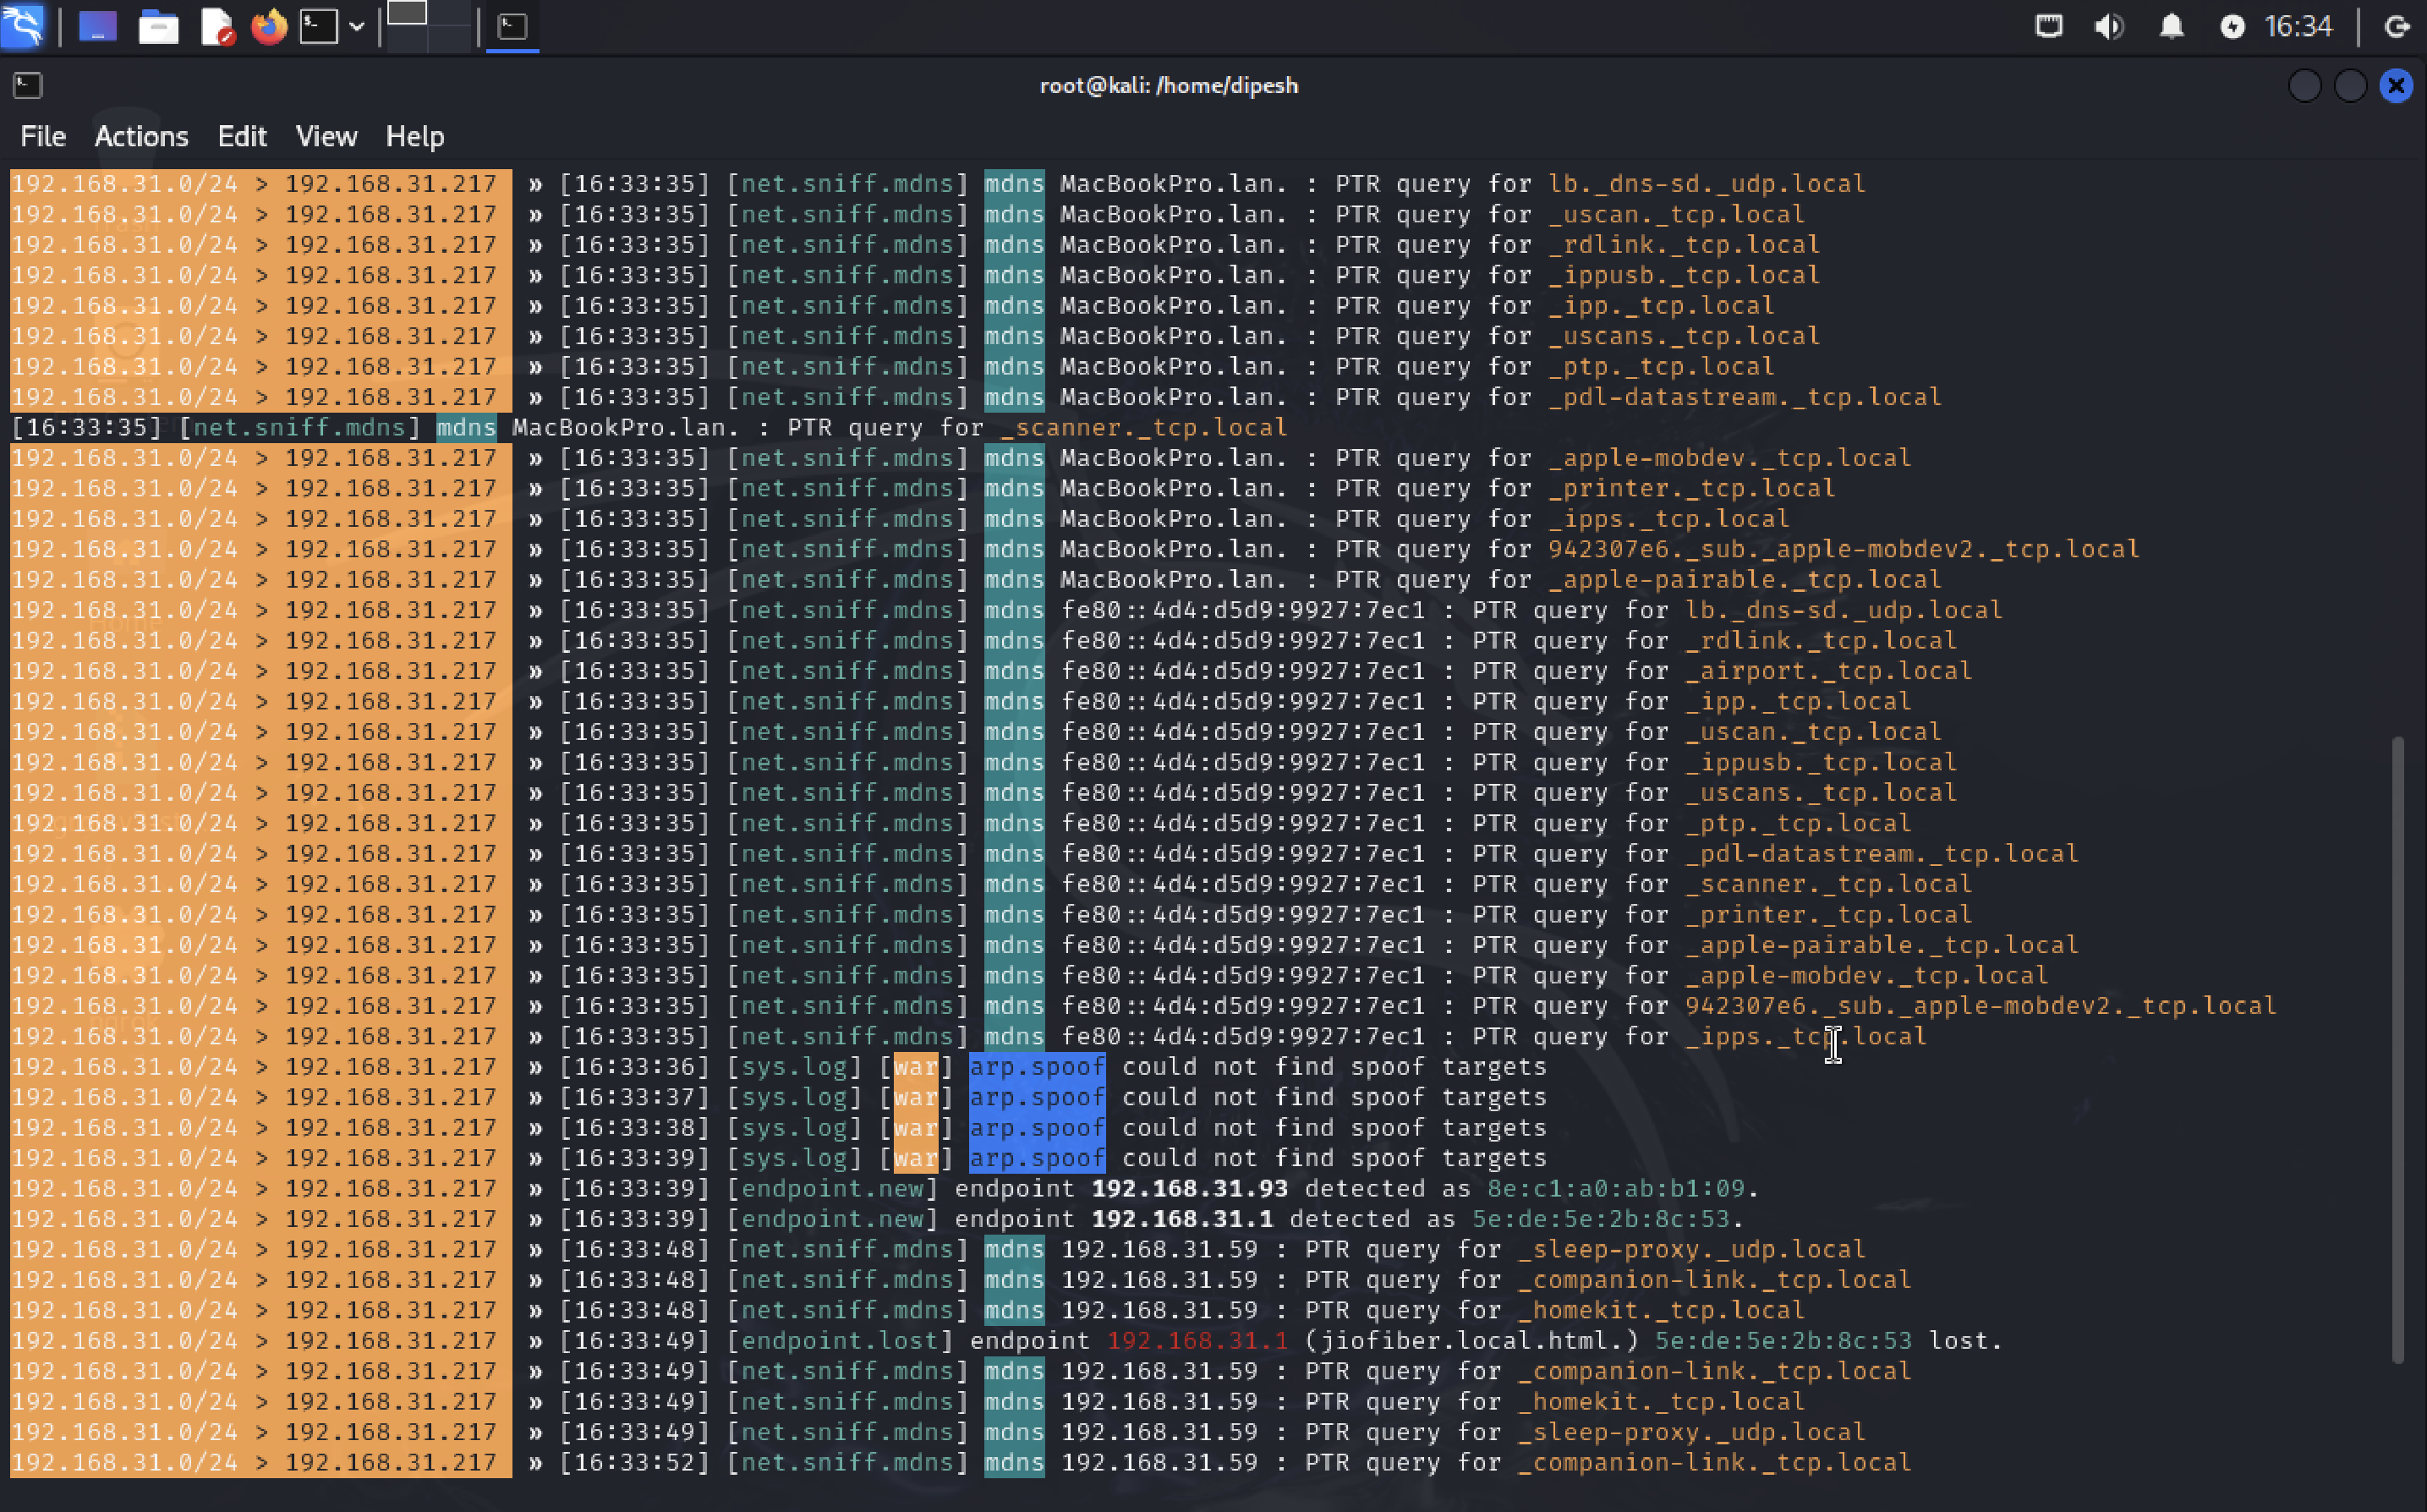
\includegraphics[width=1\linewidth]{workingofbettercap.png}
    \caption{Working of BetterCAP}
\end{figure}

\textbf{Advantages of BetterCAP:}
\\• Multiple protocols supported-HTTP, HTTPS, FTP, etc High Functionality.
\\• Modularity: Offer modules for different tasks; it is flexible and extensible for types of attacks.
\\• Friendly CLI: It is easy to perform complex tasks using simple commands for users.
\\• Being updated constantly, the version is trusted since BetterCAP is continuously being developed and updated through support from the community.
\\• Cross-platform compatibility ensures that this software runs on either Linux, macOS, and Windows, allowing flexibility.

\textbf{Disadvantages of BetterCAP:}
\\• The fact that the tool happens to be complex does make it a bit challenging for beginners to use, as its powerful features are somewhat of a steep learning curve.
\\• Legal and Ethical Issues: This software can't be used for carrying out unauthorized MITM attacks, which is illegal as well as unethical. It should be used responsibly.
\\• Limited GUI Options: It is mainly CLI-based and can be challenging for users who prefer a graphical user interface.
\\• Resource-Intensive: It is very resource-intensive in low-end systems.

\subsection{Comparision of Tools:}
HackerTarget.com had done a comparison test on various scanning tools i.e. Nessus, OpenVAS, Nexpose and NMAP. Key points on how testing was done are given below:
\\1. OpenVAS v5 scanned with the full and fast scan profile (all the ports were TCP ports and top 100 UDP ports).
\\2. Nessus v5 was launched by using the external network scan profile (also tested by internal network scan but the results were similar).
\\3. The Nexpose scanner was executed with the complete review profile.
\\4. No default scan profiles were modified.
\\5. This test was on an external network service, so no credentials were used.
\\6. This devices were scanned on a sample set of exploitable and misconfigured services on the Metasploitable framework.

\\   
\\These are the counts of vulnerabilities successfully discovered and rated by each vulnerability scanner, from the sample set of exploitable services.

\begin{figure}[h]
    \centering
    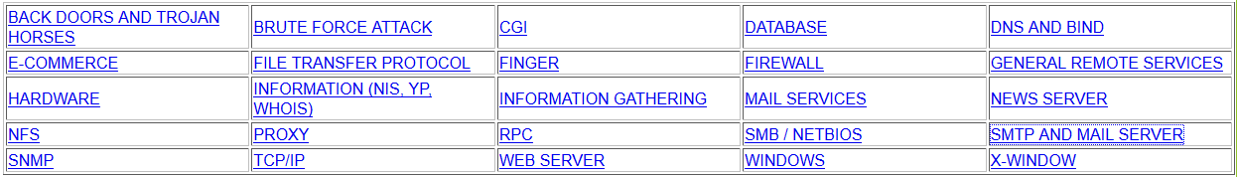
\includegraphics[width=0.5\linewidth]{image.png}
    \caption{Comparision result: Number of vulnerabilities found in each tool}
\end{figure}

\textbf{7 out of 15 security holes identified}

\section{Literature Survey}
Connections with other networks for example, the internet open up useful avenues by which the attacker can bargain for the inner end-systems. Inner network clients can inadvertently or intentionally compromise the network and its end-system through their activities. If one of the inner devices on the network has a chance of being compromised, then it becomes a threat to the rest of the network. Thus the internet as well as intranet provide convenient channels through which an attacker (either external/internal) can compromise end-systems So, Network security plays an essential role in an organization.

\subsection{Network security}
Network security defends against external and internal threats with a complete arsenal of security shields that present threats to the network. These protections include the following:
\\• Physical and environmental safeguards for network devices.
\\• Technical controls within the network infrastructure that limit its vulnerability to security threats.
\\• Controls applied within the life-cycle courses of action to utmost the vulnerability of network infrastructure to security threats.
\\• Information security operations to detect, respond to, and recover from security incidents.

Network security controls threats from outside networks basically through protections conveyed at outer network interfaces. Inside the network security perimeter, protections that are intended to detect, react to, and recover from attacks control threats from insiders and give in-depth defense against outer dangers. Network security is based on specific principles and concepts that are related to asset
protection. Let's first know some general terms and their meanings about asset protection:-

Asset : An asset is any property of value to an organization[1]. Knowing what assets need to be protected, what they are worth, where they are, and how exposed they are, an efficient amount of time, effort, and money can be spent in protecting those assets.

Vulnerability: It is the susceptibility that could be perceived as some sort of flaw or weakness in the application, through which an attacker could possibly facilitate undesirable operations or access data in a way unauthorized to them. Vicinity of vulnerability can be referred to a threat for the user of an application as it might give away sensitive information. For instance, Buffer Overflow.

\textbf{Threat :} Any form of possible danger to assets. Example:Virus

\textbf{Risk:} A risk is the chance of any given threat utilizing any specific attack against any specific system vulnerability leading to an undesired end

\textbf{Attack: } An activity set up to breach a system security policy. Example: Brute Force

\textbf{Exploit: } A series of a command or a chunk of data whose goal is the exploitation of any flaw or vulnerability of an application.

\textbf{Note: } If a vulnerability exists and there is no threat toward that vulnerability, then technically there is no risk.

At the time of designing/assessing/auditing network security, a network admin has to be aware of the following:
\\• The threats (or possible attacks) that could compromise security
\\• The cost to actualize the correct security countermeasures for a threat
\\• Cost-benefit analysis to determine if this security measure is worthwhile Implementing Now, some words associated with Network Security from this dissertation:
\\1. Network scanning
\\2. Vulnerability scanning
\\3. Penetration testing

\subsubsection{Network scanning}
Network scanning or enumeration is actually a computer program that's used to retrieve usernames, hostnames, shares, and services of networked computers. Network scanning also known as Network Security Scanner is an all-in-one networking utilities package that hosts a vast range of different tools for network monitoring and auditing network security, including vulnerability auditing, among more.
\\The program basically encompasses six modules:
\\\textbf{IP Scan:}
\\IP scanner tool to check whether a specified host can be accessed through the network. It is also used separately to check the network interface card of the computer or to check the speed. The task of ping is performed by sending the target ICMP - echo request packets and listening to ICMP - echo response. The round trip time is measured in ping; it also logs any packet lost and displays when finished a quantifiable report of the echo reply packets obtained, minimum, mean, max, and in some editions standard deviation of the round trip time.
\\\textbf{Host Scanner:}
\\It is a software designed to scan a network for open ports[2]. This is largely used by administrators to check the security of their networks. In TCP/IP protocol stack, host and host services are referred in this system using two elements: an address and a port number. The free and available port numbers are 65536. Most services use only a limited range of numbers; once the service reaches this crucial point these numbers will inevitably be obtained allocated by the IANA.

\\\textbf{Nslookup: }
\\Nslookup is a computer program in Windows and UNIX to ask the DNS servers to find details of DNS. This includes: the IP address of a given computer, MX records for a specific domain, and the NS servers of a domain. Representation of nslookup is known as "name server lookup".

\\\textbf{Traceroute :}
\\To get the path of packets over an IP network in computer network, the tool used is Traceroute. For collecting information regarding network infrastructure and IP ranges around a given host, analyzers use traceroute. It traces the path of packets to give information about network architecture. In network troubleshooting, the most frequently used tool is traceroute. Identify the path that has been taken on the network to get to a specific destination; it lets the user showing a list of routers traversed. This is used in solving routing problems or firewalls that are blocking access to a certain site. Gives list of routers traversed, which recognizes the path taken by the network to reach to a specific destination that it allows the user to do so. That helps in routing problems or firewalls that may otherwise deny access.

\\\textbf{Vulnerability Auditing :}
\\For scanning weak hosts, each known vulnerable script will try to exploit the service targeted. The fundamental point to test a host for defenseless scripts and efforts including Operating system, management, firewall, Remote Procedure Call and remote management vulnerabilities. The fundamental point is to test a host for vulnerable scripts and exploits for OS, service, firewall, Remote Procedure Call and remote management vulnerabilities.

\subsection{Vulnerability assessment}
Return information about potential security chances that allow IT staff to see the network the way a potential hacker may, clearly identifying potential roads denial of service attacks or gaining information via packet sniffing. Vulnerability scanners often prioritize weaknesses they uncover, assigning different values to represent the potential damage a hacker could cause within a network by exploiting a given weakness. This allows network administrators to point their remediation efforts in nodes that pose the largest threats.
Here following concepts of vulnerability assessment are discussed:
\\• Where vulnerability can be found i.e. area of vulnerabilities?
\\• What are type of vulnerabilities found?
\\• How this vulnerability is categorized i.e. vulnerability domains?
\\• Types of tools for performing vulnerability assessment
\\• Limitations of vulnerability assessment.

\begin{figure}[h]
    \centering
    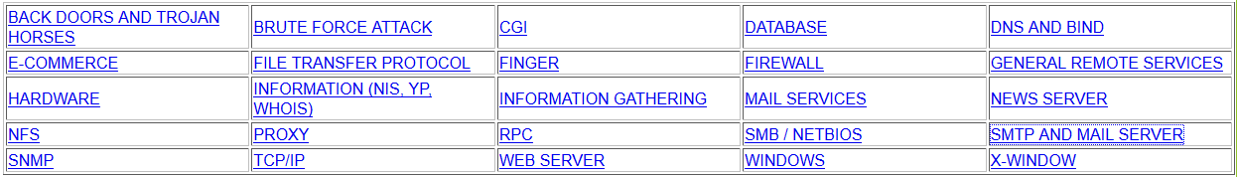
\includegraphics[width=0.5\linewidth]{image.png}
    \caption{Areas of vulnerability}
\end{figure}

\textbf{Access Control: }
Access control is the process by which users are identified and privileges granted to information, resources, and systems. The discrimination in controlling how privileges are granted and how resources are accessed ensures private and confidential information from unauthorized users. The access control mechanism should maintain and timestamp all communications and transactions so that they might be analyzed for security breaches and misuse.

\textbf{Application and Data Protection :}
It covers security issues related to the operating system, application programs, and the data. The aim is to make possible better availability of applications and data, reduce the risk of data loss, and maintain integrity of applications and data information.

\textbf{Platforms Protection :}
Platform protection involves attending to physical attacks on the client hardware. The threats include hardware tampering, theft, or destruction, and data tampering, disclosure, or destruction.

\subsubsection{Vulnerability types}
Generally, there are four types of Vulnerability:
\\• \textbf{Hardware vulnerability-} It includes vulnerability cause by physical devices-adding, removing, flooding, Traffic interrupting, physical attacks etc.
\\• \textbf{Software vulnerability-} It include software based vulnerability generated by software Deletion, modification under this logic bombs, trapdoor, Trojan horse, information leaks and Virus are come.
\\• \textbf{Data vulnerability-} It consists of data security by employing confidentiality i.e. unauthorized disclosure of a data. For more precious data communication in the system it is significant to forecast data from loss or from hacking by hacking. So, mostly we employ encryption mechanism for secure data communication. Data vulnerability consists of data loss, unauthorized access, or data hack by hackers.
\\• \textbf{Web application vulnerability-} Web applications are the most common methods nowadays to make services and information available on the internet. Lamentably, this trend has also brought an increment in the number and also complexity of vulnerabilities.

\subsubsection{Vulnerability domains}
Every vulnerability is mapped to a vulnerability category. This includes vulnerabilities, potential vulnerabilities and information gathered checks. There is a one-to-one association between a vulnerability and a vulnerability category. In case a vulnerability matches with multiple categories, the service determines which category is the best match and assigns the vulnerability to that category.

\begin{figure}[h]
    \centering
    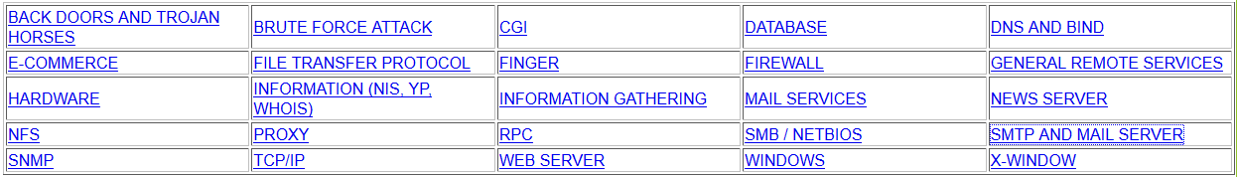
\includegraphics[width=0.5\linewidth]{image.png}
    \caption{Vulnerability Domains}
\end{figure}

\subsubsection{Types of vulnerability assessment scanner}
\\There are two kinds of VA scanners:
\\\textbf{Active Scanners :} \\Active scanners send probes to the nodes in the network, checking the responses they receive to determine if a given node is a weak point within the net work. An active scanner may be utilized by a network administrator to demonstrate an attack against the network, demonstrating weaknesses a hacker might identify, or to analyze a node after an attack to understand how a hacker exploited broke through security. Active scanners may take an action to selfrulingly address security threats, such as blocking an IP address that may potentially be dangerous.
\\\textbf{Passive Scanners: }\\All active operating systems, applications and ports that are there in the network can be detected with passive scanners. It continually scans the activities and puts attention on the weak spots of the network. Still, although the passive scan provides information on the vulnerabilities, it is incapable of doing any remedial measures regarding the security violation. These scanners can report on the current software and patch versions on networked devices, which can report what devices are using software that demonstrates a potential entryway for hackers or trojan attacks, and can reference this information against open databases containing lists of current patches. A network administrator can set passive scanners to run constantly or to work at specified interim.

\subsubsection{Comparison between network scanning, vulnerability assessment and penetration testing}

Network Scanning consists of network utilities. It doesn't actually represent hole in network but the consequence of vulnerability or attack. A vulnerability assessment is the methodology of identifying and quantifying vulnerabilities in network. It is an in-depth assessment of network posture, demonstrating shortcomings and giving the suitable mitigation techniques needed to either take out those shortcomings
or reduce them to an acceptable level of risk. To achieve this, most vulnerability assessments follow these general steps:
\\1. Identification of resources and assets within the network
\\2. Assigning measurable value and energy to the resources
\\3. Determining the vulnerabilities or potential risks against each resource
\\4. Mitigating or eliminating the most critical vulnerabilities to the most valuable resources

Conversely, a penetration test emulates the behavior of an outside and/or inside attacker expecting to breach the security of an organization. Using many tools and techniques, the penetration tester tries to exploit critical systems and gain access to sensitive information. Depending on the level, a pen test can extend beyond the network to include social engineering attacks or physical security tests.
The basic difference in approach between a vulnerability assessment and penetration test. A vulnerability assessment answers the question: "What are our weaknesses and how do we fix them?" A penetration test basically answers the questions: "Can someone break-in and what can they attain?".
A vulnerability assessment tries to improve security action and build a more developing, integrated security program in as much as a pen test is only an instance of security program's fitness. Based on its strategy, a vulnerability assessment will produce much more respect than a pen test for the majority of efforts.

\subsection{Working principle of the Application:}
The Network Scanner App is a Kivy-based Python application that performs various network-related tasks using the nmap, netifaces, and scapy libraries. The app provides a graphical user interface (GUI) for network scanning, open port detection, service enumeration, vulnerability scanning, and packet sniffing.

\textbf{a) User Interface (UI) Flow:}\\
i. The Kivy framework is used to create a GUI with buttons for each functionality.\\
ii. The user interacts with buttons to initiate network operations.
The app opens popups to accept user input (e.g., an IP address or subnet range).\\
iii. After execution, results are displayed in popup windows.

\textbf{b) Core Functionalities:-}\\

\textbf{*) Network Scanning:}\\
i. Uses netifaces to determine the local network range.\\
ii. Uses nmap to ping scan the network (-sn argument).\\
iii. Identifies live devices, extracting their IP, MAC addresses, and hostnames.\\
iv. Displays the result in a popup window.\\

\textbf{*) Open Port Scanning:}\\
i. Accepts a target IP address from the user.\\
ii. Uses nmap with the -sS argument for TCP SYN scan.\\
iii. Detects open ports and their corresponding services.\\
iv. Displays the list of open ports in a popup.\\

\textbf{*) Service Enumeration:}\\
i. Accepts a network range from the user.\\
ii. Uses nmap -sV to detect running services and their versions.\\
iii. Lists active services along with port numbers.\\
iv. Displays results in a popup window.\\

\textbf{*) Vulnerability Scanning:}\\
i. Accepts a target IP address.\\
ii. Uses nmap --script vuln to run vulnerability detection scripts.\\
iii. Identifies possible security weaknesses in the target.\\
iv. Displays the vulnerability report in a popup.\\

\textbf{*) HTTP and HTTPS Packet Sniffing:}\\
i. Accepts an IP address from the user.\\
ii. Uses Scapy's sniff() function to capture HTTP or HTTPS packets.\\
iii. Extracts raw payload data from HTTP packets.\\
iv. For HTTPS packets, extracts domain names using regex.\\
v. Displays captured packets in a popup.\\

\textbf{c) Execution Flow:-}\\
i. User opens the application.\\
ii. Selects a feature from the UI.\\
iii. If needed, enters an IP or subnet.\\
iv. The app executes the corresponding network operation.\\
v. Results are processed and displayed in a popup.\\

\textbf{d) Tools and Libraries Used:-}\\
\begin{table}[h]
    \centering
    \begin{tabular}{|l|p{6cm}|} % Adjust column width
        \hline
        \textbf{Library} & \textbf{Purpose} \\
        \hline
        \texttt{kivy} & GUI Development (Buttons, Popups, Layouts) \\
        \hline
        \texttt{nmap} & Network Scanning (Host Discovery, Port Scanning, Service Detection) \\
        \hline
        \texttt{netifaces} & Getting Local Network Details (IP Address, Subnet Mask) \\
        \hline
        \texttt{scapy} & Packet Sniffing (Capturing HTTP/HTTPS Traffic) \\
        \hline
    \end{tabular}
    \caption{Libraries and Their Purposes}
    \label{tab:libraries} 
\end{table}

\textbf{e) Security Considerations:-}\\
i. Requires administrative privileges for scanning and sniffing.\\
ii. Scanning networks without permission is illegal in many places.\\
iii. Using packet sniffing on unauthorized networks can be a privacy violation.\\

\section{OVERARCHING OBJECTIVE:}
The general goal of the Advanced Network Scanner project is to improve network security by integrating several open-source scanning tools (NMAP, OpenVAS, and BetterCAP) into one easy-to-use interface. The scanner should:\\

i) Detect Active Hosts: Discover devices within a network, identify their operating systems, installed software, and configurations.\\
ii) Detect Vulnerabilities: Evaluate network security by comparing information against a signature database of known vulnerabilities.\\
iii) Automate Threat Surveillance: Ongoing scanning for infected devices and configuration errors.\\
iv) Facilitate Security Analysis: Report faster and more in-depth vulnerability scans with less manual effort and scanning time.\\
v) Enhance Usability: Provide a user-friendlier interface than traditional command-line-based scanners.\\
\begin{figure}[h]
    \centering
    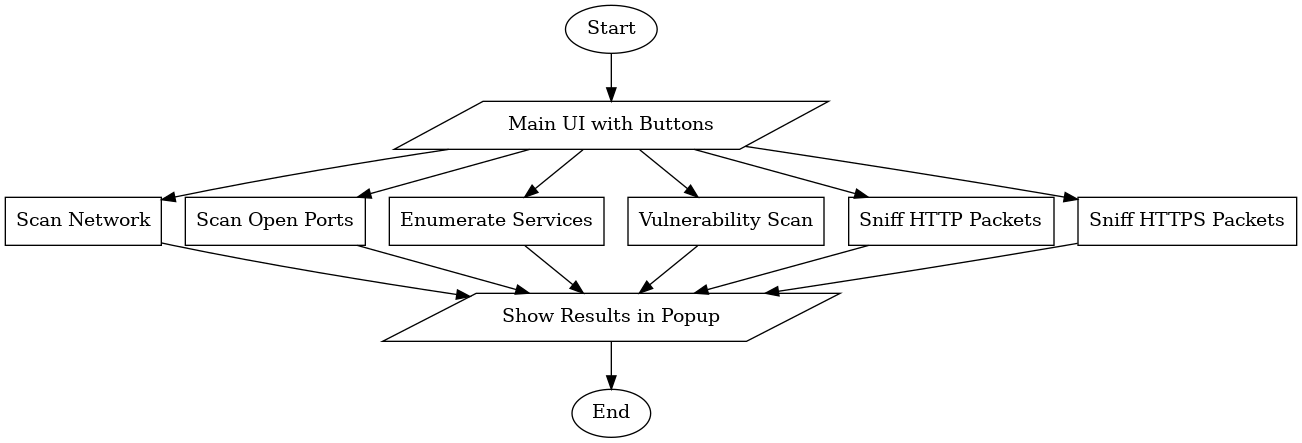
\includegraphics[width=1\linewidth]{network_scanner_flowchart.png}
    \caption{flow chart}
    \label{fig:enter-label}
\end{figure}

\section{RESULTS:}[h]
\begin{figure}[h]
    \centering
    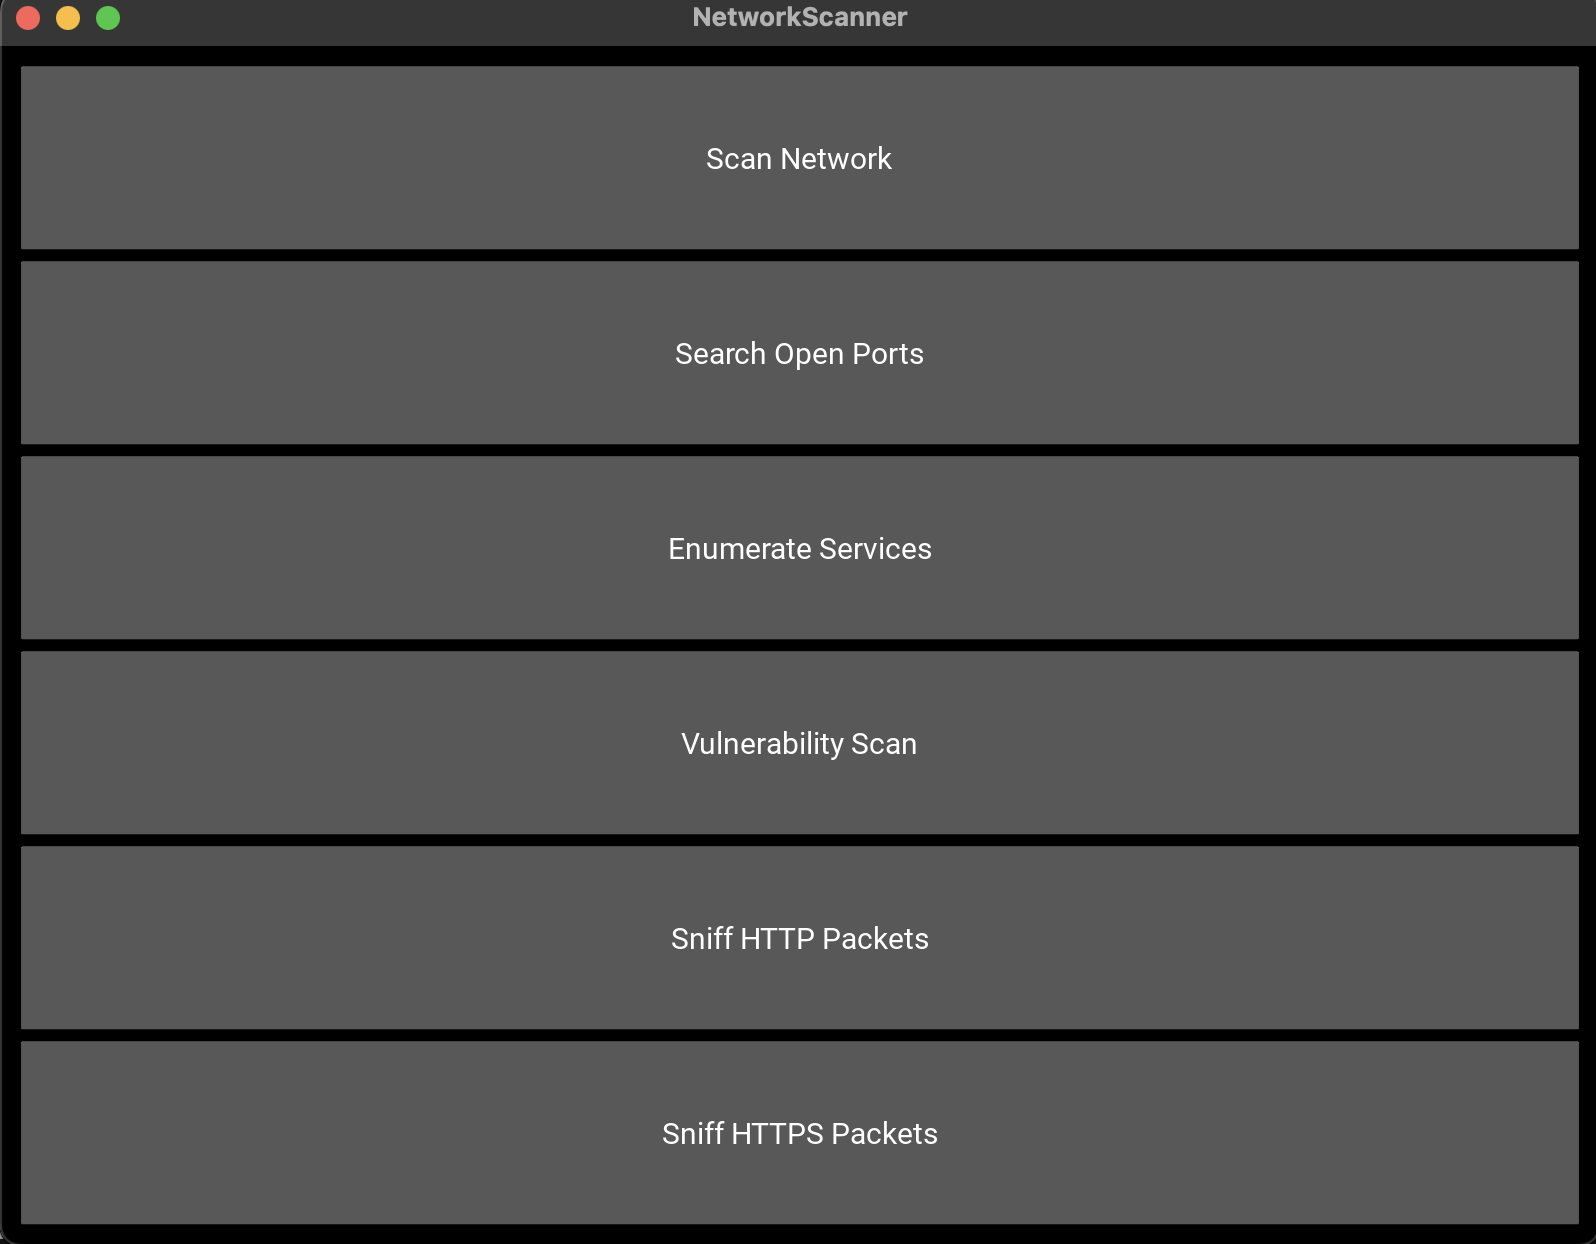
\includegraphics[width=0.75\linewidth]{r0.png}
    \caption{interface}
    \label{fig:enter-label}
\end{figure}
\\
\begin{figure}[h]
    \centering
    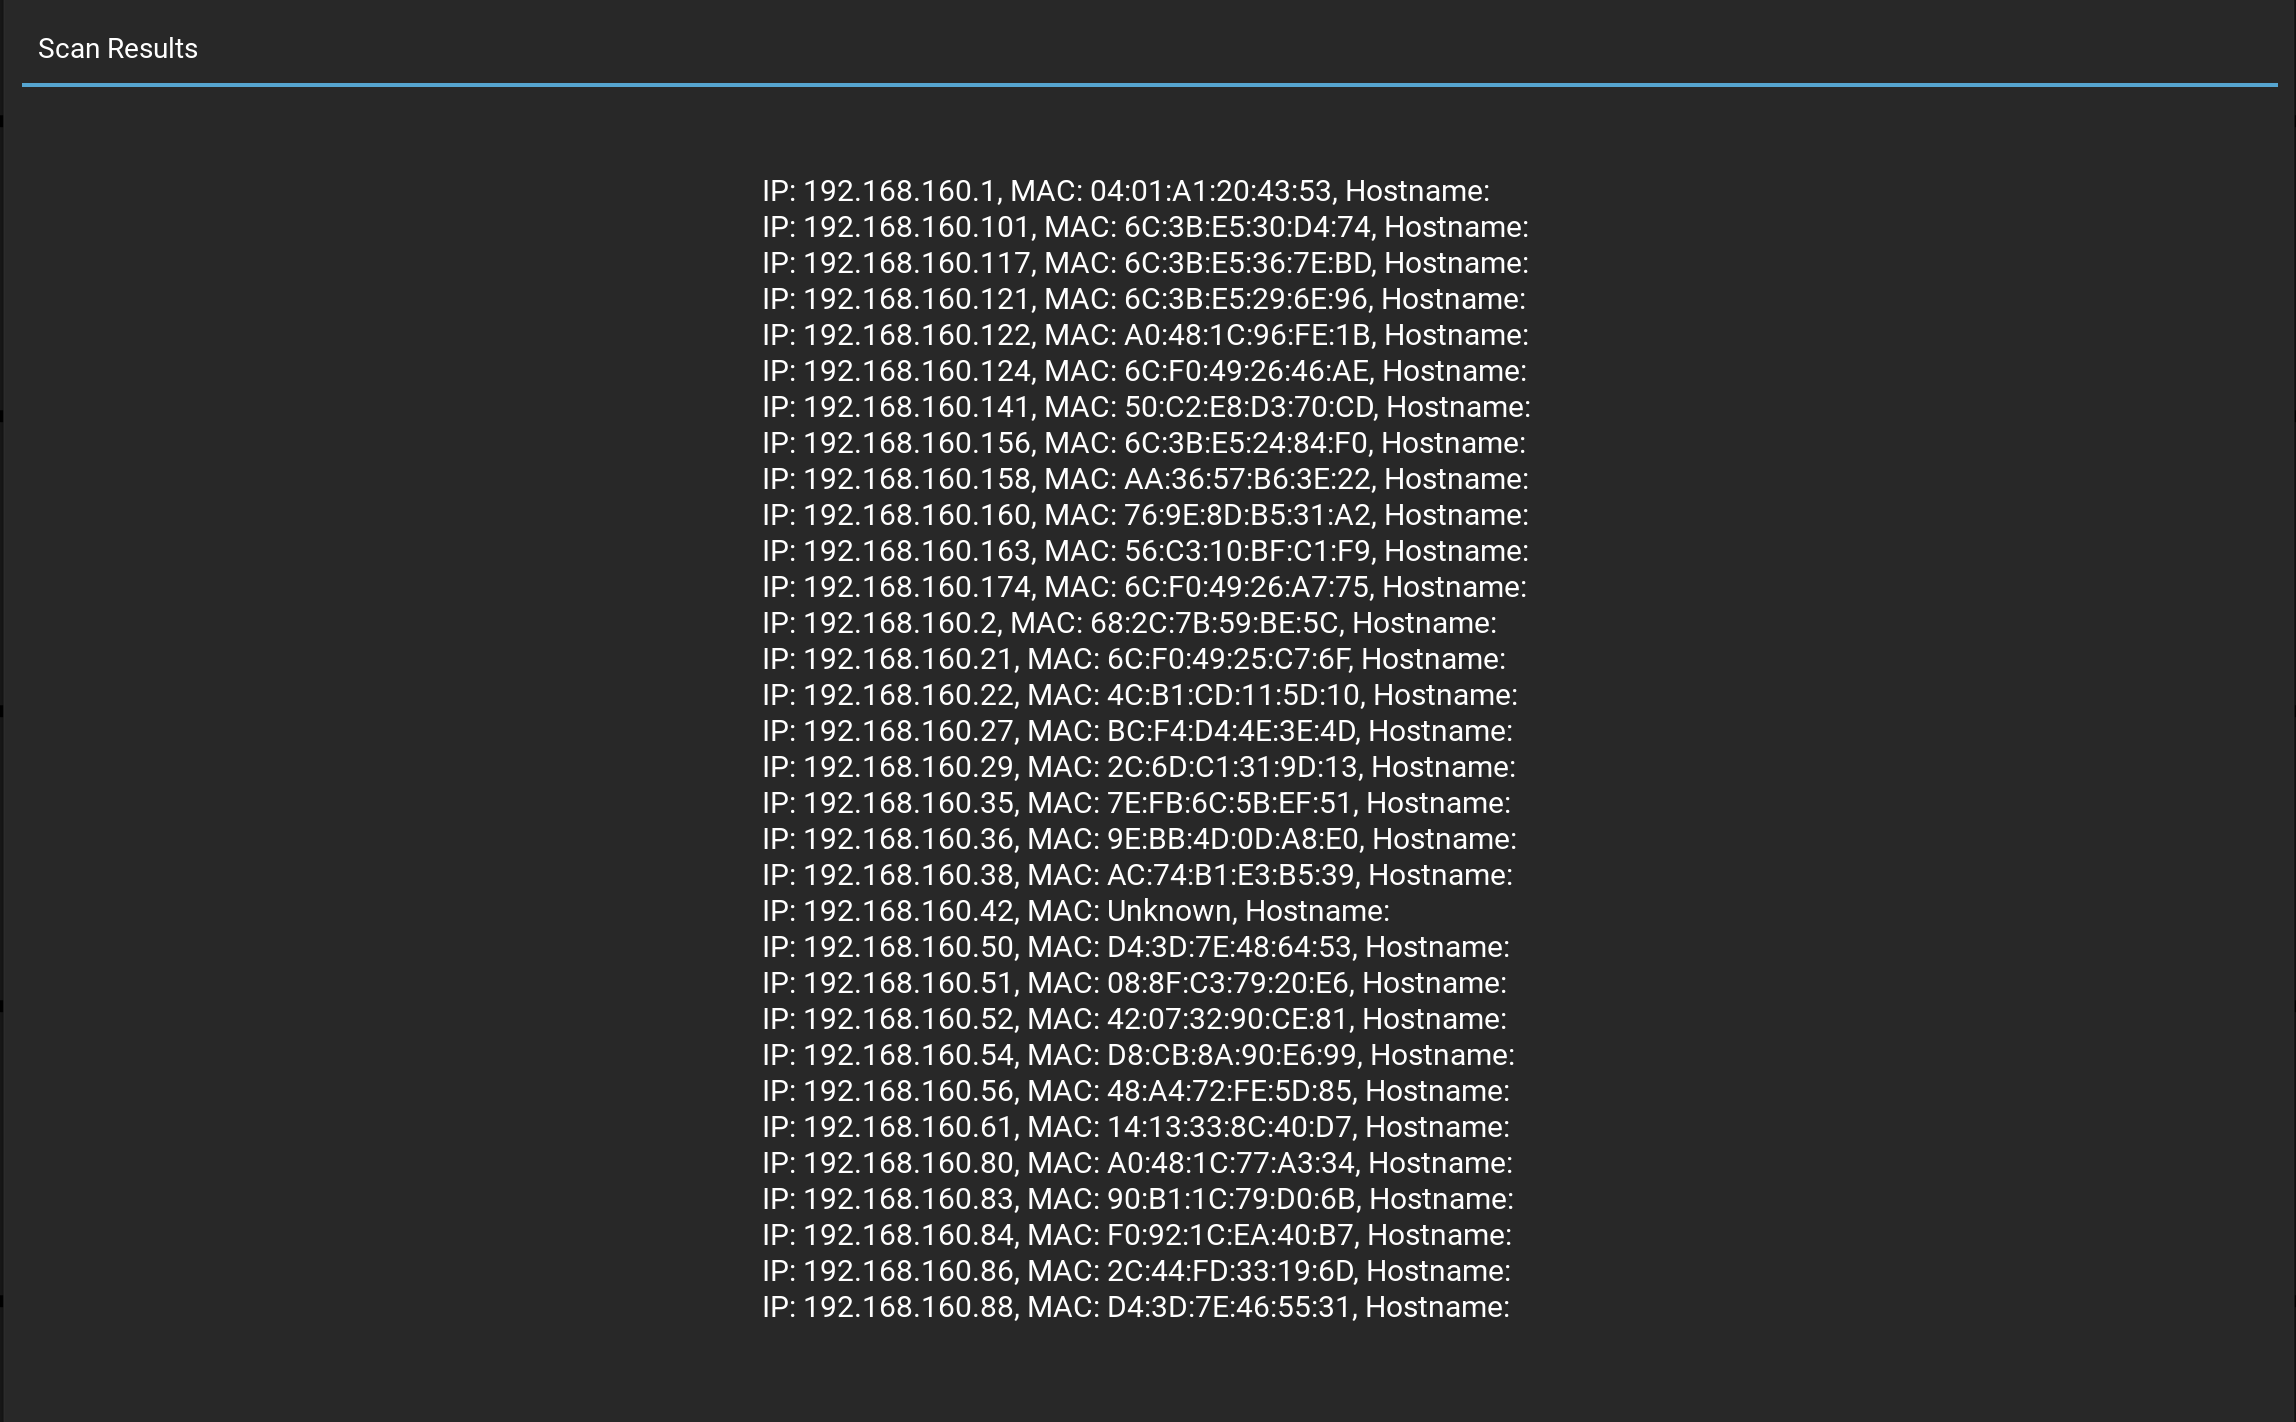
\includegraphics[width=1\linewidth]{r.png}
    \caption{scan network}
    \label{fig:enter-label}
\end{figure}
\begin{figure}[h]
    \centering
    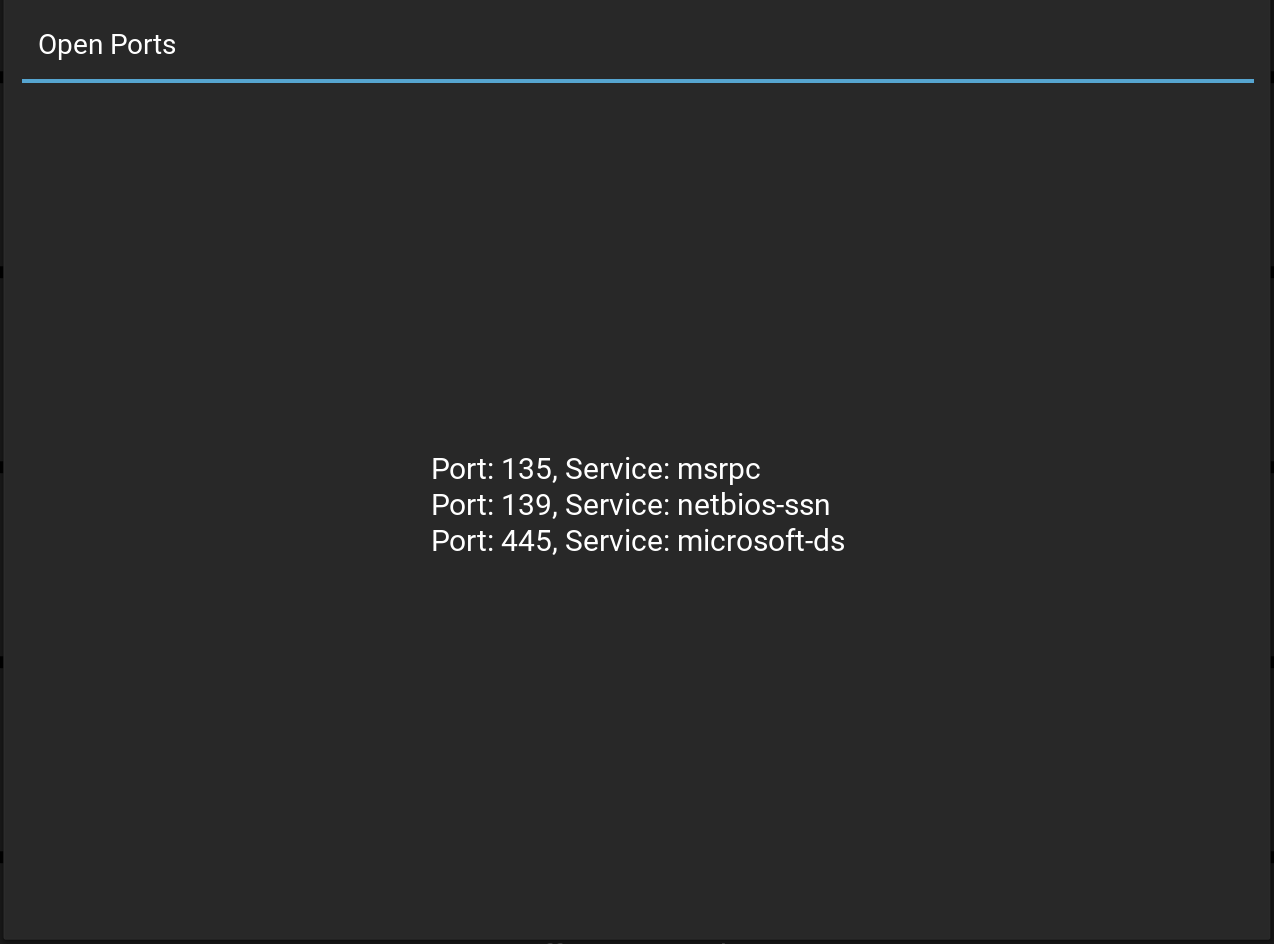
\includegraphics[width=1\linewidth]{r2.png}
    \caption{open ports}
    \label{fig:enter-label}
\end{figure}
\begin{figure}[h]
    \centering
    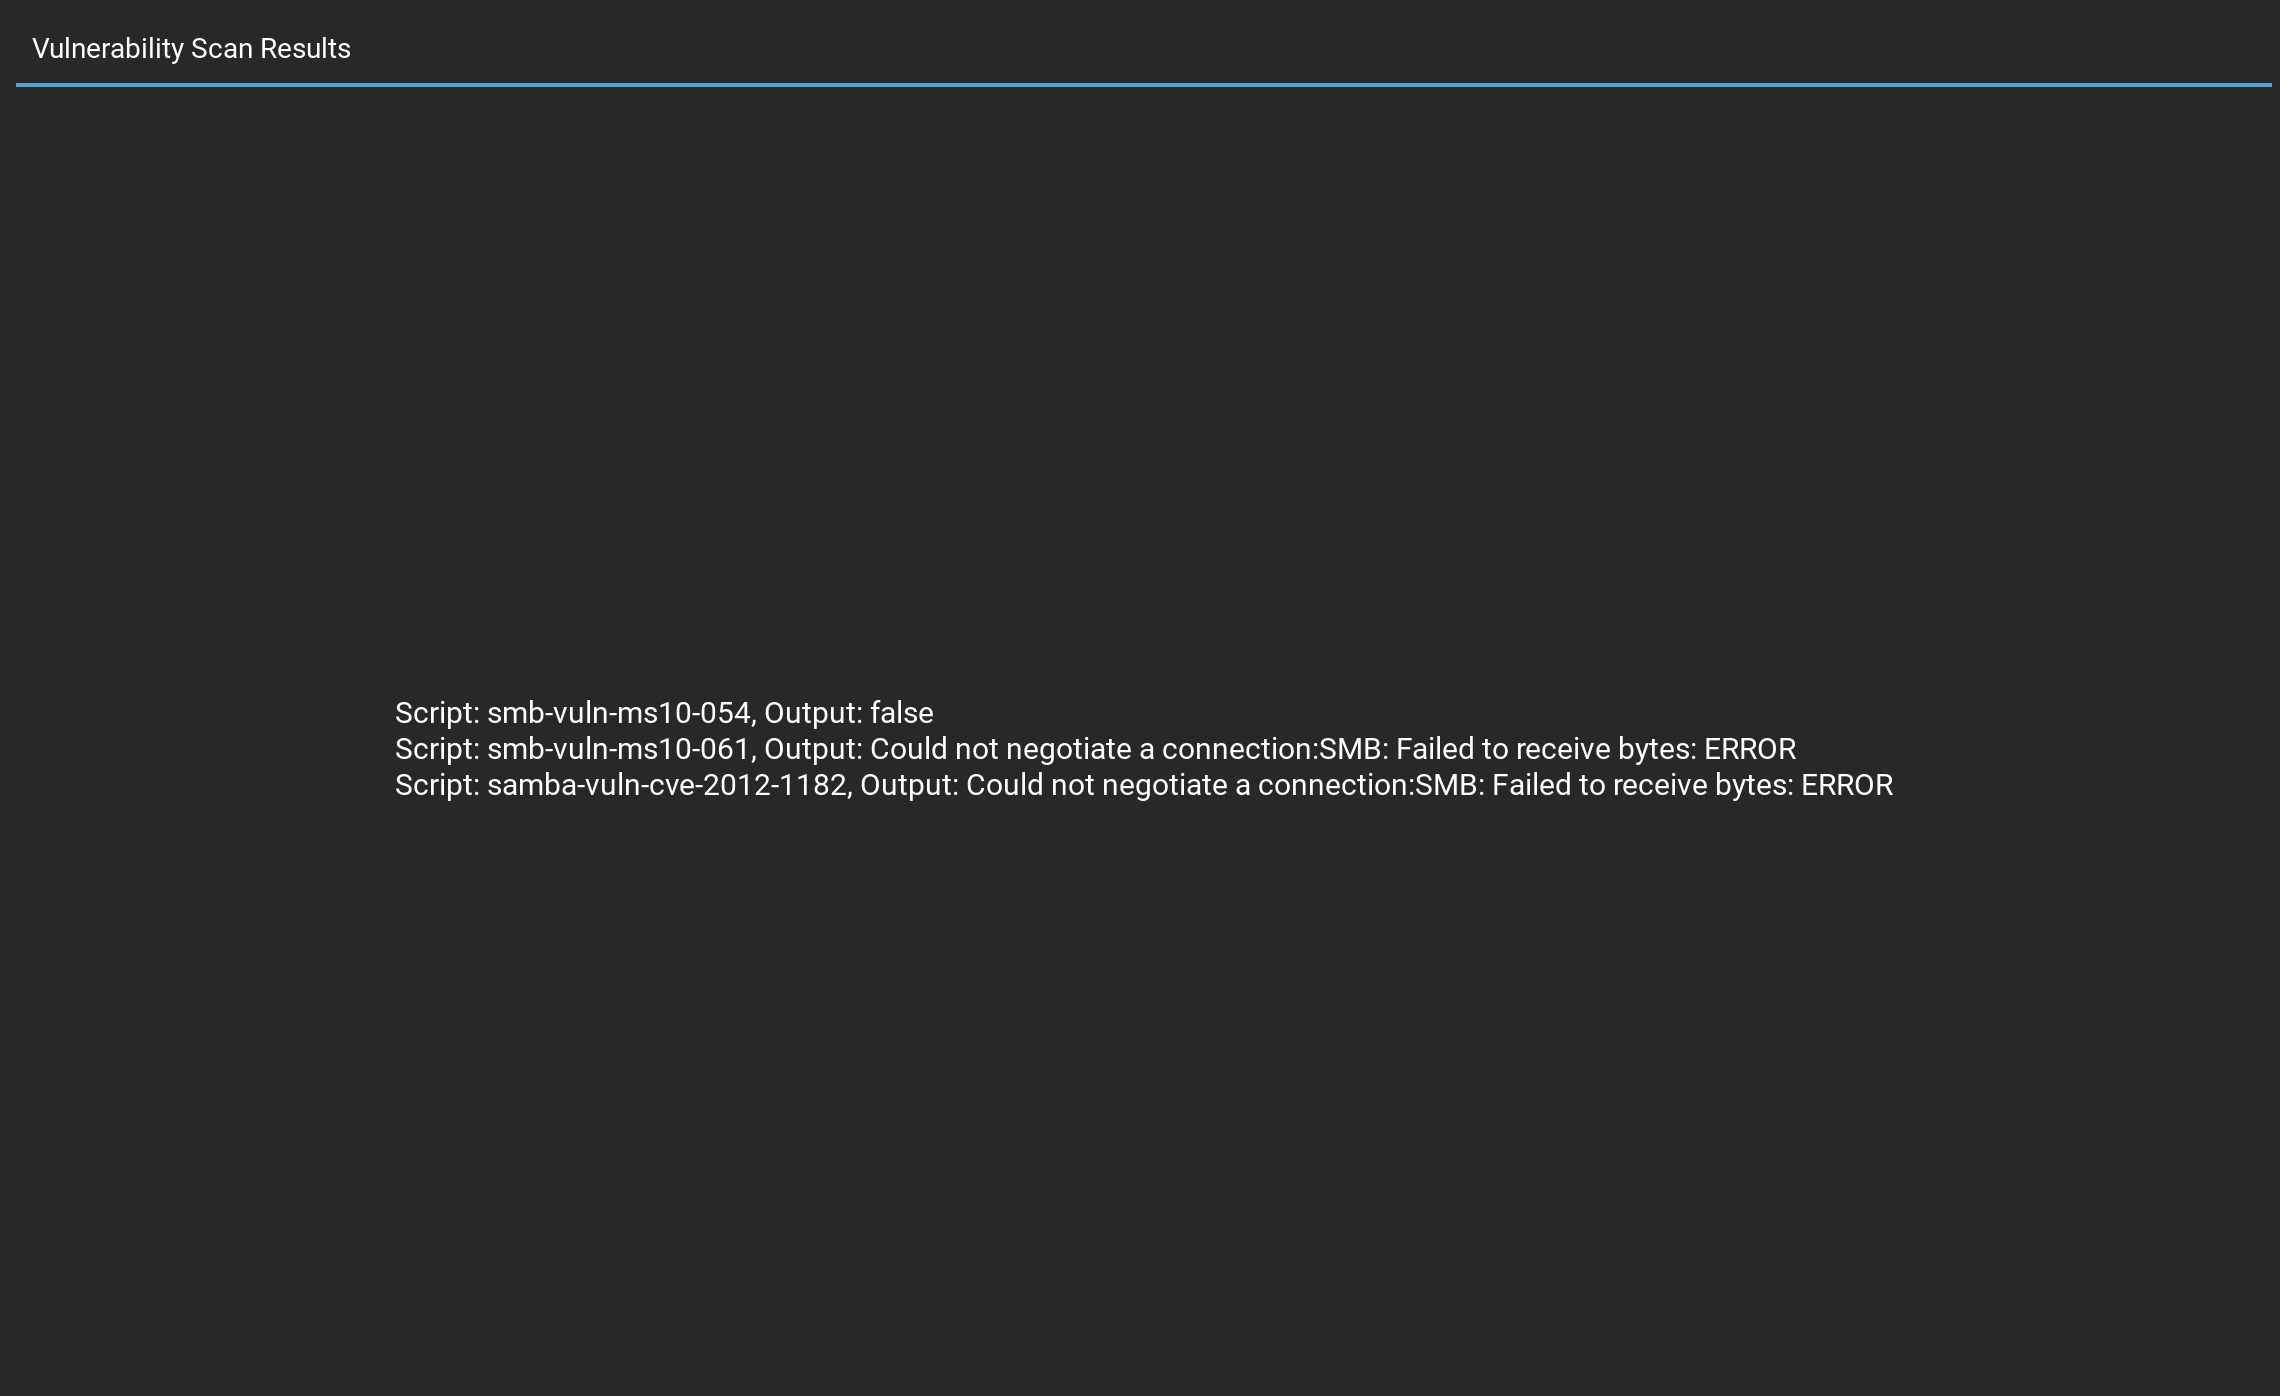
\includegraphics[width=1\linewidth]{r3.png}
    \caption{vulnerability}
    \label{fig:enter-label}
\end{figure}
\begin{figure}[h]
    \centering
    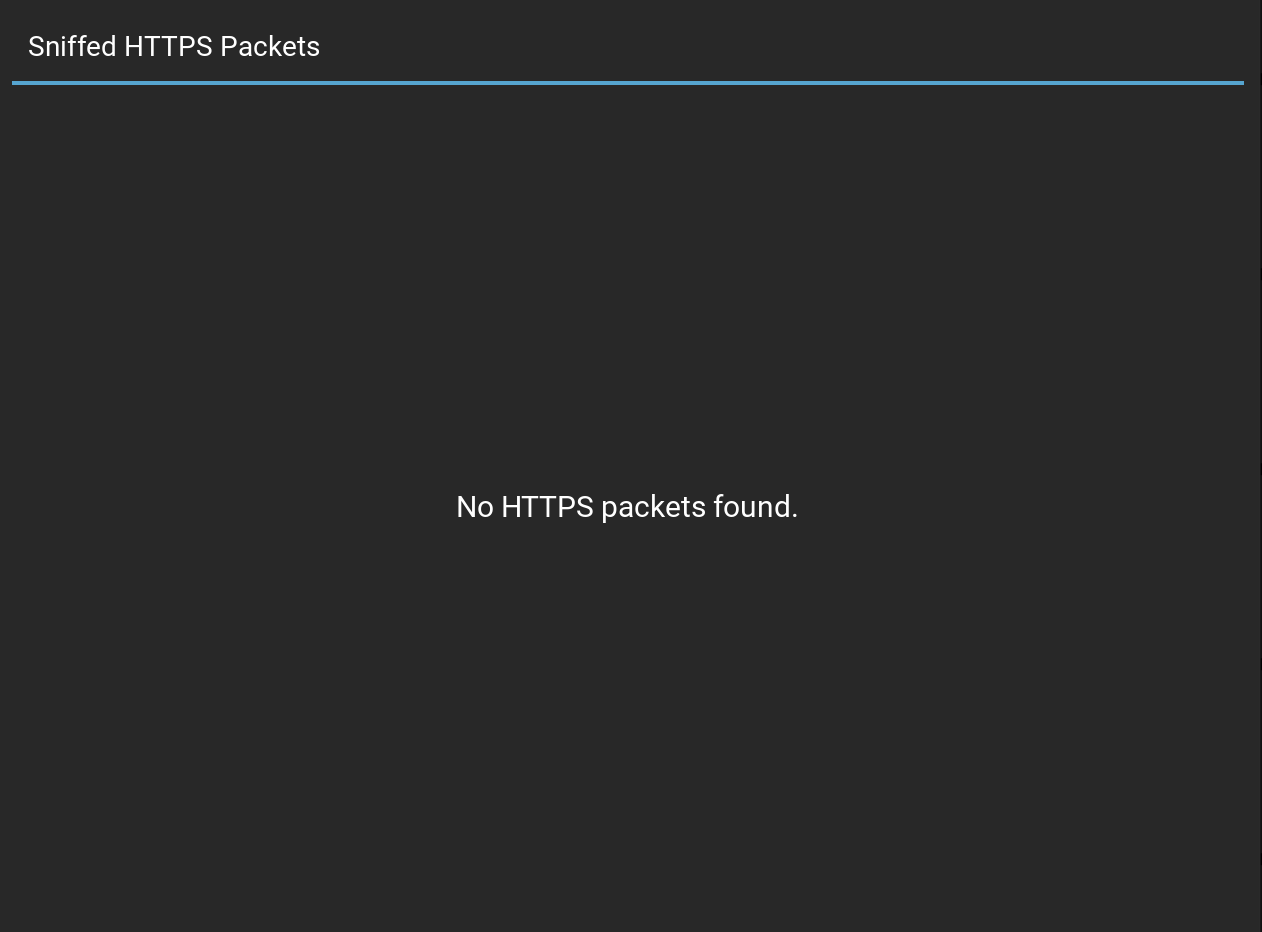
\includegraphics[width=1\linewidth]{r4.png}
    \caption{https packet}
    \label{fig:enter-label}
\end{figure}
\begin{figure}[h]
    \centering
    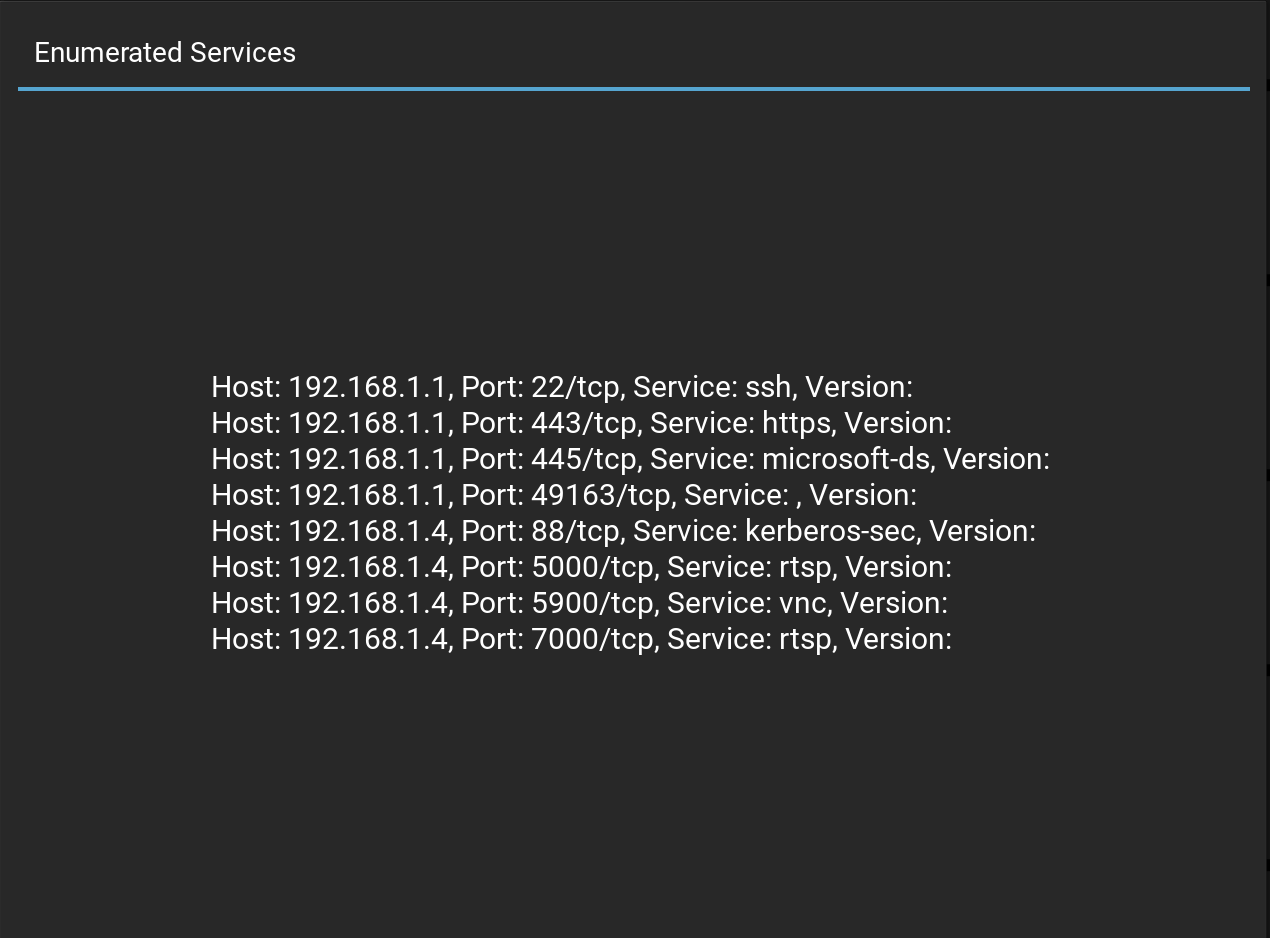
\includegraphics[width=1\linewidth]{r5.png}
    \caption{service enumeration}
    \label{fig:enter-label}
\end{figure}

\section{Conclusion:}{h}
The Advanced Network Scanner efficiently integrates a number of open-source tools (NMAP, OpenVAS, and BetterCAP) to provide a single network security tool. By incorporating the features of these tools, the scanner enhances network vulnerability scanning, active host discovery, enumeration of services, and automated threat detection.

The key contributions of this project are:\\

i) Efficient Network Scanning: Identifies active devices, open ports, and running services.\\
ii) Vulnerability Detection: Cross-matches collected data against a vulnerability database to detect security threats.\\
iii) Automated Monitoring: Enables continuous scanning of compromised devices, reducing security response time.\\
iv) User-Friendly Interface: Consolidates complex functionality of NMAP, OpenVAS, and BetterCAP into a simple GUI.\\
Despite these advantages, some limitations are the complexity of processing heterogeneous data from diverse tools and legal/ethical issues with network scanning. Future directions can involve machine learning-based anomaly detection, real-time security alerts, and cloud-based network scanning in large-scale environments.


\begin{thebibliography}{9}
    \bibitem{NmapBook}
    Lyon, G. \textit{Nmap Network Scanning: The Official Nmap Project Guide to Network Discovery and Security Scanning}. 
    This book offers in-depth knowledge about Nmap's capabilities in network scanning, which aligns with your project's goal of integrating Nmap's features.

    \bibitem{NmapDoc}
    Nmap Official Documentation. 
    Covers all of Nmap’s features and extensions, such as OS detection, version scanning, and scriptable interactions with services. Exploring Zenmap (Nmap’s GUI) could also provide ideas for a user-friendly interface.

    \bibitem{OpenVASDoc}
    OpenVAS User Manual and Admin Guide. 
    Essential for understanding its vulnerability assessment capabilities, including the OpenVAS Scanner and Manager, which handle large-scale vulnerability assessments.

    \bibitem{OpenVASResearch}
    \textit{Security Vulnerability Detection and Monitoring using OpenVAS and Virtual Lab Environment}. 
    This research paper can offer insights into OpenVAS's integration in secure environments.

    \bibitem{BetterCAPRepo}
    BetterCAP GitHub Repository. 
    Contains the source code and information on various modules that allow for traffic interception, injection, and network manipulation.

    \bibitem{BetterCAPDoc}
    BetterCAP Documentation. 
    Extensive documentation on its modular features, particularly useful for implementing man-in-the-middle attacks, packet sniffing, and ARP spoofing.

    \bibitem{HackingExposed}
J. Scambray, S. McClure, and G. Kurtz, \textit{Hacking Exposed 7: Network Security Secrets \& Solutions}. McGraw-Hill Education, 2012.

\bibitem{TaoNetworkSecurity}
R. Bejtlich, \textit{The Tao of Network Security Monitoring: Beyond Intrusion Detection}. Addison-Wesley Professional, 2004.

\bibitem{NmapGuide}
G. Lyon (Fyodor), \textit{Nmap Network Scanning: The Official Nmap Project Guide to Network Discovery and Security Scanning}. Nmap Project.

    \bibitem{SommerML}
R. Sommer and V. Paxson, "Outside the Closed World: On Using Machine Learning for Network Intrusion Detection," \textit{IEEE Symposium on Security and Privacy}, 2010.

\bibitem{ScalasVulnScan}
M. Scalas, L. Francioso, and P. Peretti, "A Comprehensive Analysis of Open-Source Network Vulnerability Scanners," \textit{IEEE Access}, 2021.

\bibitem{UllrichIDS}
J. Ullrich, P. Barford, and V. Paxson, "Network Intrusion Detection: Evasion, Traffic Morphing, and Malicious Automation," \textit{ACM Transactions on Information and System Security}, 2016.

\bibitem{MITRE}
MITRE, "MITRE ATT\&CK Framework," Available at: \url{https://attack.mitre.org/}.

\bibitem{CVE}
CVE, "Common Vulnerabilities and Exposures Database," Available at: \url{https://cve.mitre.org/}.

\bibitem{OWASP}
OWASP, "Open Web Application Security Project," Available at: \url{https://owasp.org/}.

    
\end{thebibliography}



\end{document}
